\section{Resultados}
En esta sección se presentan los resultados descriptivos y de los análisis estadísticos de las eficiencias de los ICB cuando se tiene cada uno de los casos de supuestos (NVC, NNVC, NVD, NNVD), por esquema, tamaño de muestra y tipo de modelo.\\



\subsection{Eficiencia de los intervalos Bootstrap para el caso EP-NVC}
Con base en el promedio general (Figura \ref{fig:EficPromIntBootsTamMuestEsqRemuEP-NVC}) para: Eficiencia del ICB Percentil (Efic Int Boot Perc) y Eficiencia del ICB BCa (Efic Int Boot Bca) el mejor esquema resultó Liu2, 0.9569 y 0.9586 respectivamente;
Eficiencia del ICB Percentil cuando solo él lo contiene a la $R^{2}$ y Eficiencia del ICB BCa cuando solo él contiene a la $R^{2}$ el mejor esquema es Liu1, 0.7354 y 0.7366 respectivamente;
la Eficiencia de ICB Percentil cuando gana en el empate a ICB BCa (Efic Boot Perc gana empate), el mejor esquema es Wu1 $(0.8989)$ y la Eficiencia ICB BCa cuando gana en el empate al ICB Percentil (Efic Boot Bca gana empate), el mejor esquema es Wu3 $(0.4304)$.\\

%Poner el contexto
Sin considerar el tamaño de la muestra y esquema, para el caso EP-NVC los ICB mejores en promedio general (Figura \ref{fig:EficPromIntBootsTamMuestEsqRemuEP-NVC}) son: el ICB Percentil con $0.8091$ ante la Eficiencia en ICB BCa; la Eficiencia del ICB Bca cuando solo él contiene a la $R^{2}$ $(0.1516)$ y la Eficiencia de ICB Percentil cuando gana en el empate al ICB Bca con $0.7047$. Por lo que, el mejor es ICB Percentil.\\


\begin{figure}[H] 
	\centering 
	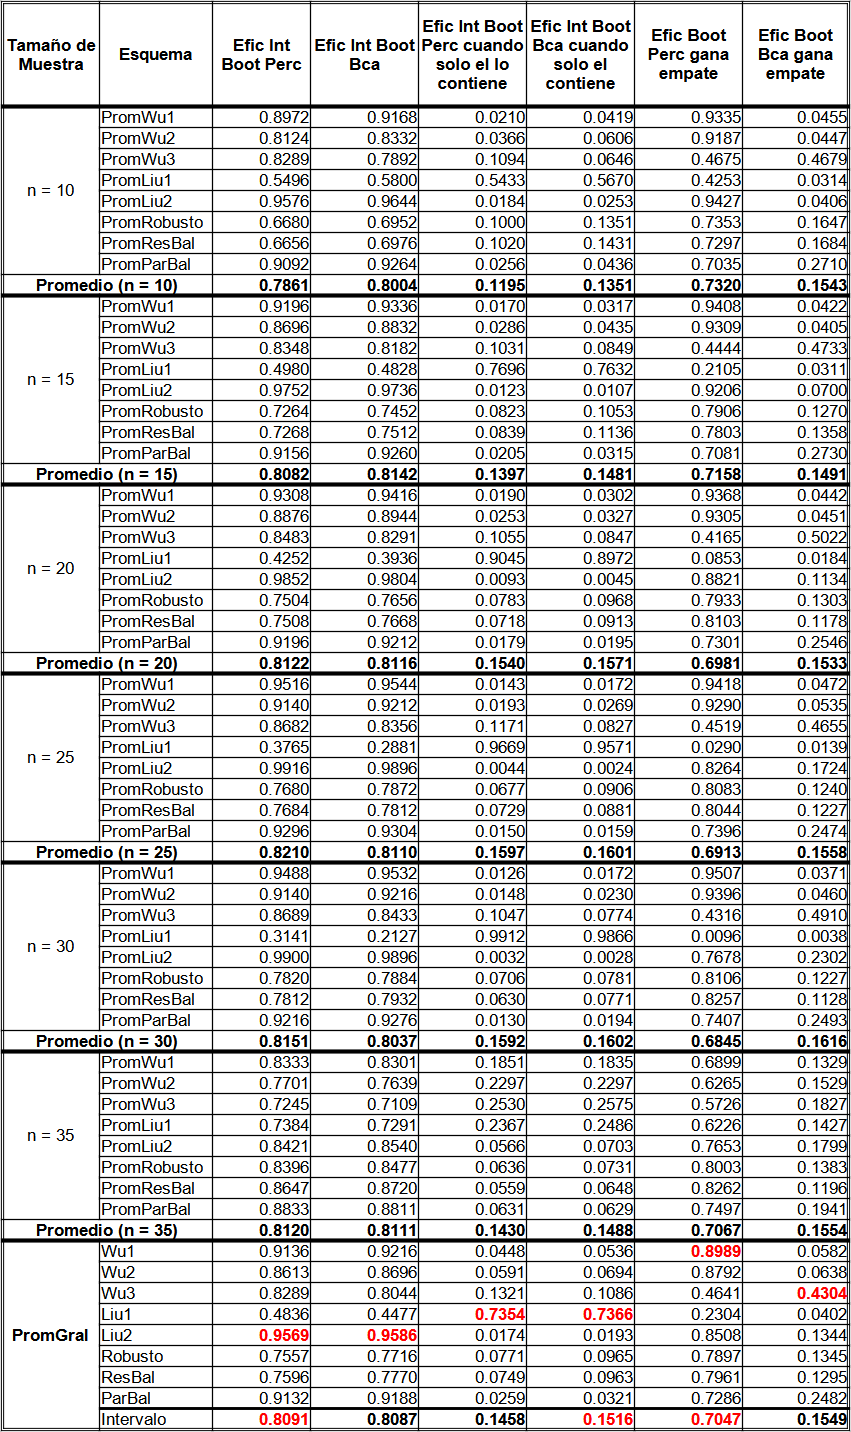
\includegraphics[width=0.55\linewidth]{img/EP_NVC_Efic_Boots.png} 
	\caption{Eficiencia promedio de los intervalos Bootstrap por tamaño de muestra y esquema de remuestreo para el caso EP-NVC.} 
	\label{fig:EficPromIntBootsTamMuestEsqRemuEP-NVC}
\end{figure}

\FloatBarrier

\subsubsection{Eficiencia de los esquemas para el caso EP-NVC}
Con base en al menos 95\% de eficiencia promedio y sin importar el ICB  (Figura \ref{fig:EficPromEsqTamMuesEsqRemuEP-NVC}): $n=10$ ningún esquema cumplió la condición, sin embargo con Liu2 se obtuvo 0.94, y con los tamaños de muestra 15, 20, 25, 30 y 35 el mejor fue el esquema Lui2.\\


Sin considerar el tamaño de la muestra e ICB, para el caso EP-NVC el mejor promedio general (Figura \ref{fig:EficPromEsqTamMuesEsqRemuEP-NVC}) en eficiencia de esquema es Liu2 (0.9737).


\begin{figure}[H] 
	\centering 
	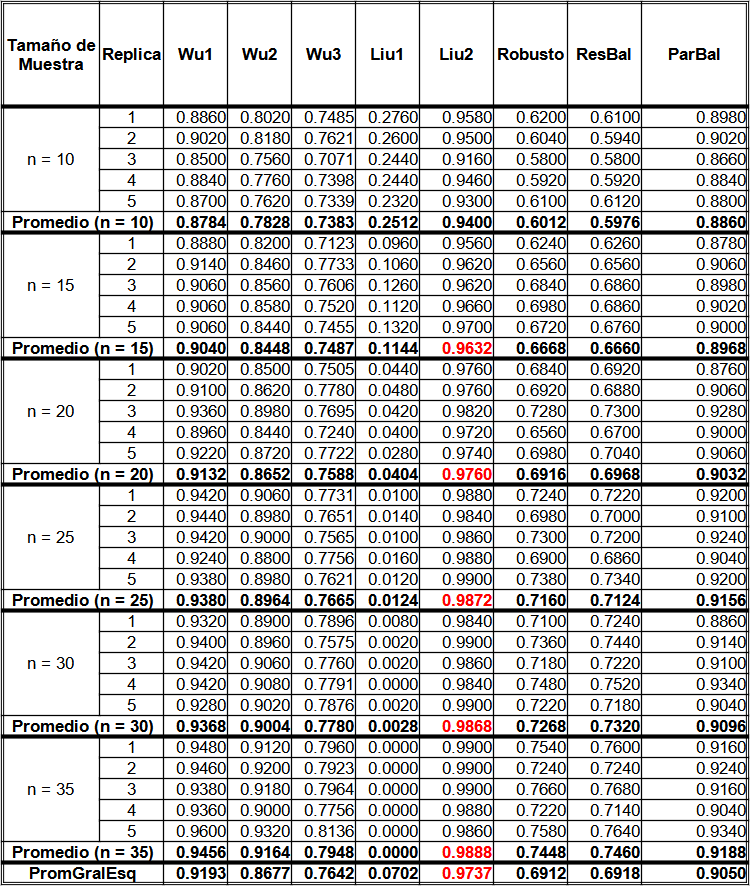
\includegraphics[width=0.70\linewidth]{img/EP_NVC_Efic_Esq.png} 
	\caption{Eficiencia promedio de los esquemas por tamaño de muestra para el caso EP-NVC.} 
	\label{fig:EficPromEsqTamMuesEsqRemuEP-NVC}
\end{figure}

\FloatBarrier

%%%%%%%%%%%%%%%%%%%%%%%%%%%%%%%%%%%%%%%%%%%
\subsection{Eficiencia de los intervalos Bootstrap para el caso EP-NNVC}
Con base en el promedio general (Figura \ref{fig:EficPromIntBootsTamMuestEsqRemuEP-NNVC}) para: Eficiencia del ICB Percentil (Efic Int Boot Perc) y Eficiencia en ICB BCa (Efic Int Boot Bca) el mejor esquema resultó Liu2, 0.9893 y 0.9870 respectivamente;
Eficiencia del ICB Percentil cuando solo él contiene a la $R^{2}$ y Eficiencia del ICB BCa cuando solo él contiene a la $R^{2}$ el mejor esquema es Liu1, 0.6381 y 0.6549 respectivamente; 
la Eficiencia de ICB Percentil cuando gana en el empate a ICB BCa (Efic Boot Perc gana empate), el mejor esquema es Wu2 $(0.9026)$ y la Eficiencia ICB BCa cuando gana el empate al ICB Percentil (Efic Boot Bca gana empate), el mejor esquema es Wu3 $(0.8147)$.\\


Sin considerar el tamaño de la muestra y esquema, para el caso EP-NNVC los ICB mejores en promedio general  (Figura \ref{fig:EficPromIntBootsTamMuestEsqRemuEP-NNVC}) son: Eficiencia del ICB BCa (Efic Int Boot Bca) con $0.8653$ ante $0.8604$ de la Eficiencia en ICB Percentil (Efic Int Boot Perc); la Eficiencia del ICB BCa cuando solo el contiene a la $R^{2}$ $(0.1117)$ y la Eficiencia de ICB Percentil cuando gana en el empate al ICB BCa (Efic Boot Perc gana empate) con $0.6697$. Por lo que, el mejor es ICB Percentil.



\begin{figure}[ht] 
	\centering 
	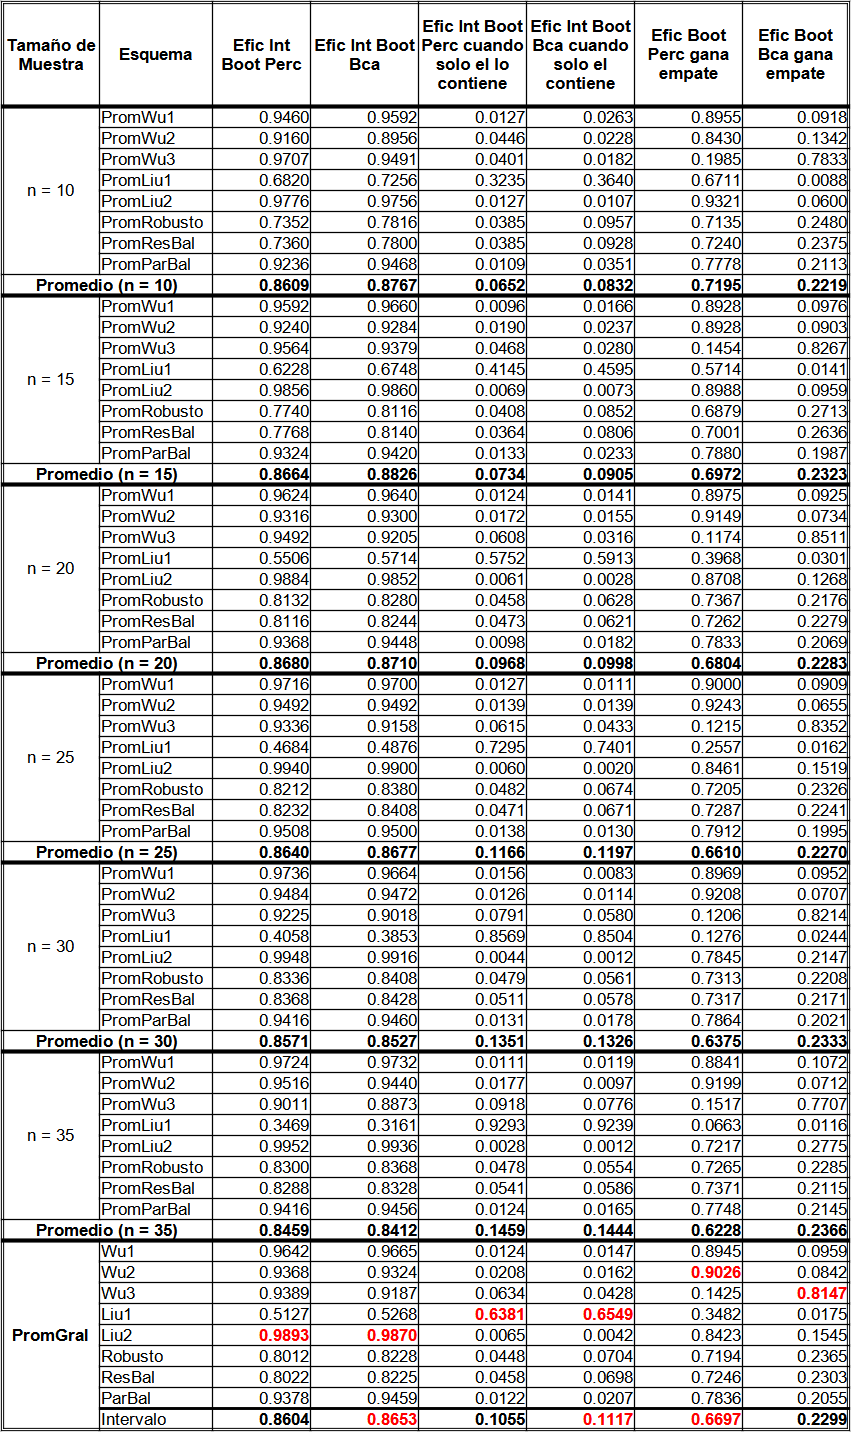
\includegraphics[width=0.55\linewidth]{img/EP_NNVC_Efic_Boots.png} 
	\caption{Eficiencia promedio de los intervalos Bootstrap por tamaño de muestra y esquema de remuestreo para el caso EP-NNVC.} 
	\label{fig:EficPromIntBootsTamMuestEsqRemuEP-NNVC}
\end{figure}
\FloatBarrier


\subsubsection{Eficiencia de los esquemas para el caso EP-NNVC}
Con base en al menos 95\% de eficiencia promedio y sin importar el ICB (Figura \ref{fig:EficPromEsqTamMuesEsqRemuEP-NNVC}) : con $n=10$ el mejor fue el esquema Liu2 (0.9651), seguido por Wu1 (0.9340) y con los tamaños de muestra 15, 20, 25, 30 y 35 los mejores esquemas son Liu2 y Wu1.\\

Sin considerar el tamaño de la muestra e ICB, para el caso EP-NNVC los mejores promedio generales (Figura \ref{fig:EficPromEsqTamMuesEsqRemuEP-NNVC}) en eficiencia son los esquema Liu2 y Wu1.


\begin{figure}[ht] 
	\centering 
	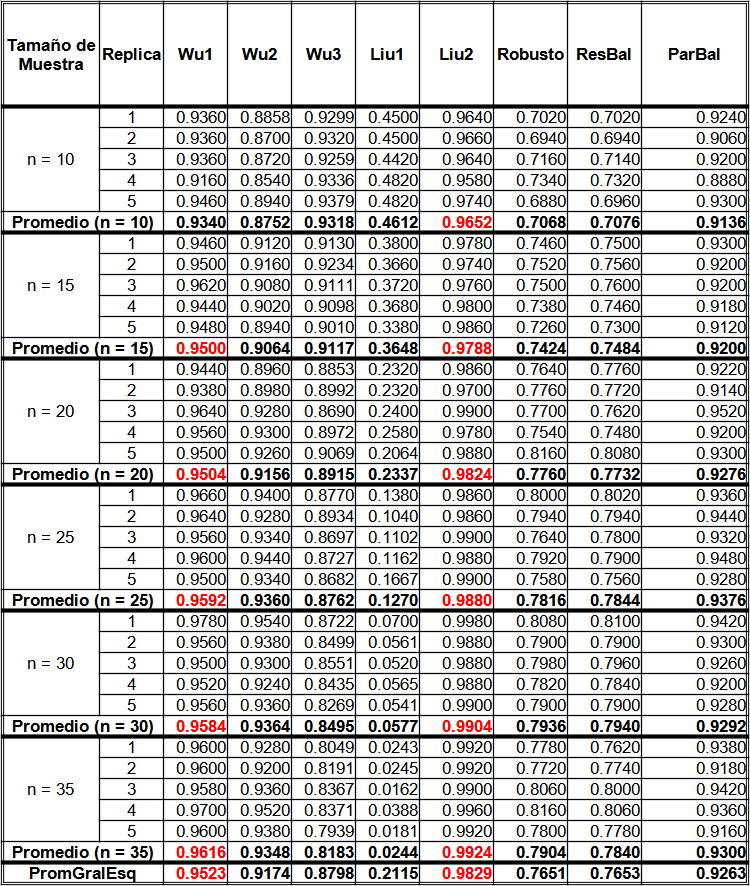
\includegraphics[width=0.70\linewidth]{img/EP_NNVC_Efic_Esq.png} 
	\caption{Eficiencia promedio de los esquemas por tamaño de muestra para el caso EP-NNVC.} 
	\label{fig:EficPromEsqTamMuesEsqRemuEP-NNVC}
\end{figure}
\FloatBarrier


%%%%%%%%%%%%%%%%%%%%%%%%%%%%%%%%%%%%%%%%%%%%%%%%

\subsection{Eficiencia de los intervalos Bootstrap para el caso EP-NVD}
Con base en el promedio general (Figura \ref{fig:EficPromIntBootsTamMuestEsqRemuEP-NVD}) para: Eficiencia del ICB Percentil (Efic Int Boot Perc) y Eficiencia en ICB BCa (Efic Int Boot Bca) el mejor esquema resultó Liu2, 0.9775 y 0.9760 respectivamente; Eficiencia del ICB Percentil cuando solo él contiene a la $R^{2}$ y Eficiencia del ICB BCa cuando solo él contiene a la $R^{2}$ el mejor esquema es Liu1, 0.5042 y 0.4677 respectivamente; 
la Eficiencia de ICB Percentil cuando gana en el empate a ICB BCa (Efic Boot Perc gana empate), el mejor esquema es Pareado Balanceado (ParBal) con 0.8230 y la Eficiencia ICB BCa cuando gana el empate al ICB Percentil, el mejor esquema es Wu3 $(0.5159)$.\\


Sin considerar el tamaño de la muestra y esquema, para el caso EP-NVD los ICB mejores en promedio general (Figura \ref{fig:EficPromIntBootsTamMuestEsqRemuEP-NVD}) son: Eficiencia del ICB BCa (Efic Int Boot Bca) con $0.8299$ ante la Eficiencia de $0.8279$ en ICB Percentil (Efic Int Boot Perc); la Eficiencia del ICB Percentil cuando solo el contiene a la $R^{2}$ $(0.1049)$ y la Eficiencia de ICB Percentil cuando gana en el empate al ICB Bca con $0.6110$. Por lo que, el mejor es ICB Percentil.\\


\begin{figure}[ht] 
	\centering 
	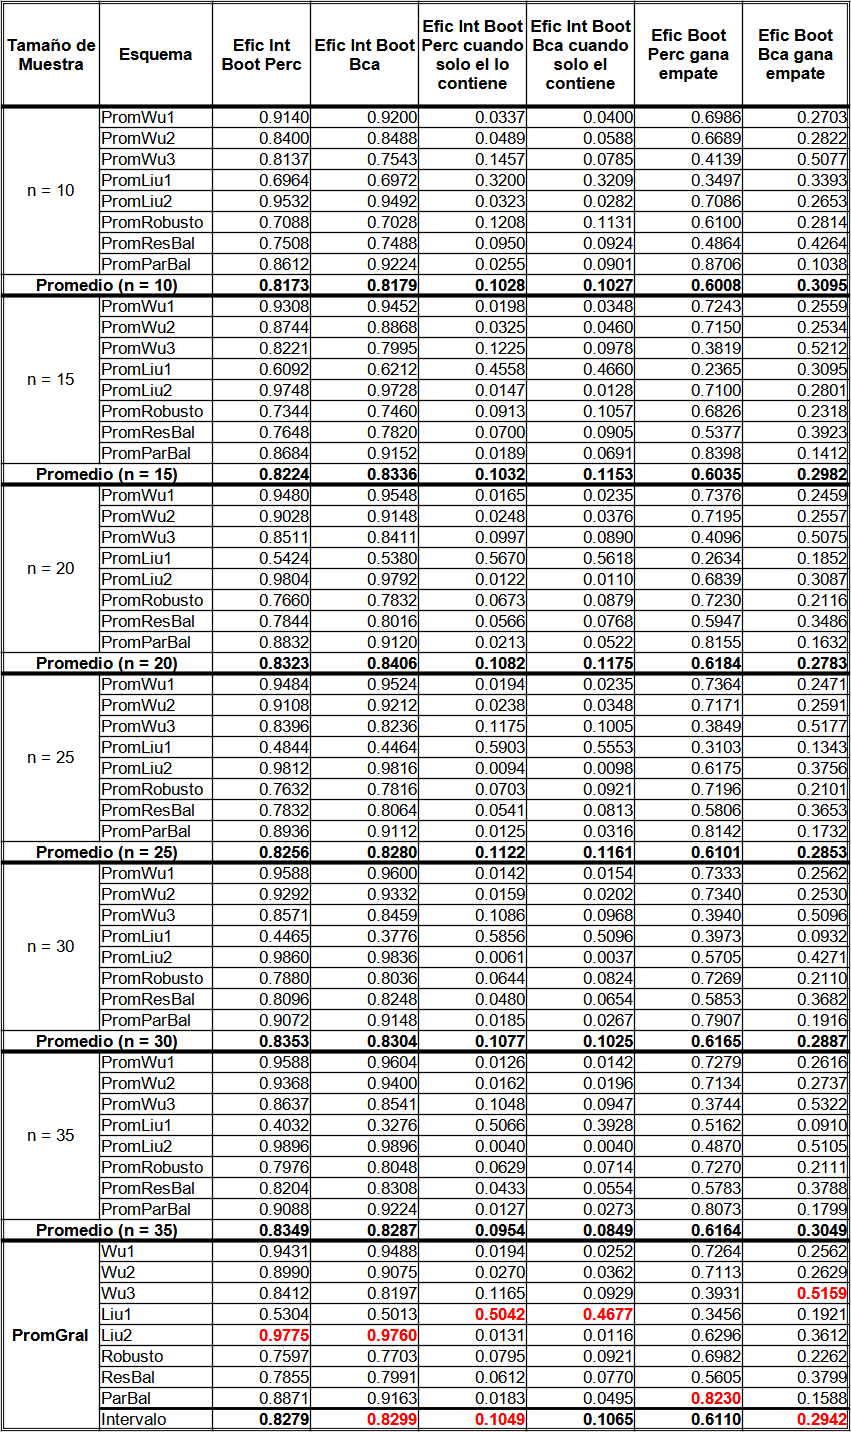
\includegraphics[width=0.55\linewidth]{img/EP_NVD_Efic_Boots.png} 
	\caption{Eficiencia promedio de los intervalos Bootstrap por tamaño de muestra y esquema de remuestreo para el caso EP-NVD.} 
	\label{fig:EficPromIntBootsTamMuestEsqRemuEP-NVD}
\end{figure}
\FloatBarrier

\subsubsection{Eficiencia de los esquemas para el caso EP-NVD}
Con base en al menos 95\% de eficiencia promedio y sin importar el ICB  (Figura \ref{fig:EficPromEsqTamMuesEsqRemuEP-NVD}): con $n=10$ ningún esquema cumplió la condición, sin embargo con Liu2 se obtuvo 0.9224 y con los tamaños de muestra 15, 20, 25, 30 y 35 el mejor fue el esquema Lui2.\\

Sin considerar el tamaño de la muestra, para el caso EP-NVD el mejor promedio general (Figura \ref{fig:EficPromEsqTamMuesEsqRemuEP-NVD}) en eficiencia por esquema es Liu2 (0.9648).


\begin{figure}[ht] 
	\centering 
	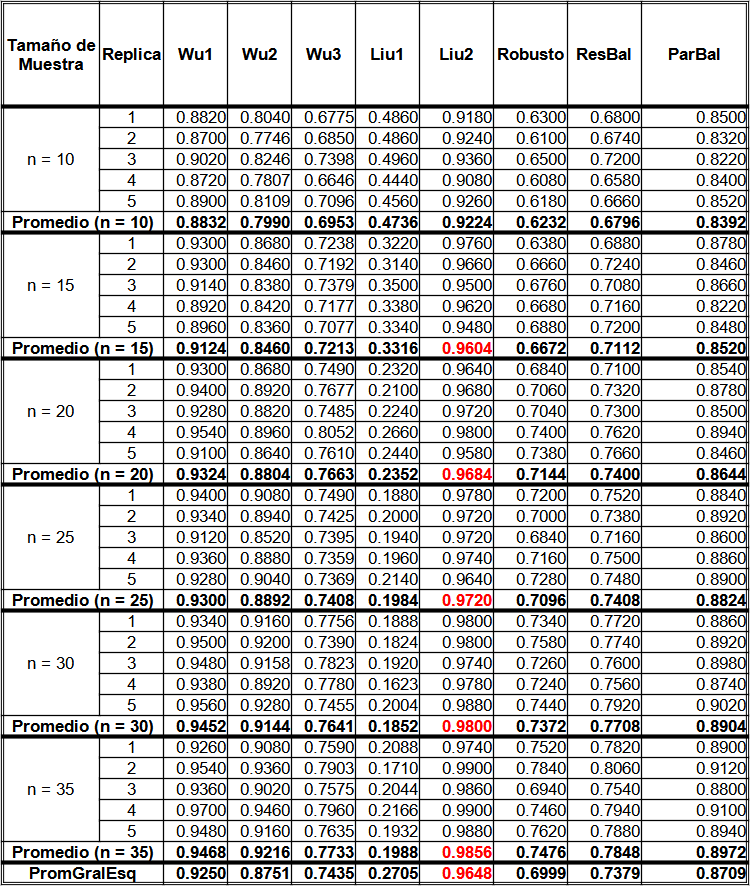
\includegraphics[width=0.70\linewidth]{img/EP_NVD_Efic_Esq.png} 
	\caption{Eficiencia promedio de los esquemas por tamaño de muestra para el caso EP-NVD.} 
	\label{fig:EficPromEsqTamMuesEsqRemuEP-NVD}
\end{figure}
\FloatBarrier


%%%%%%%%%%%%%%%%%%%%%%%%%%%%%%%%%

\subsection{Eficiencia de los intervalos Bootstrap para el caso EP-NNVD}
Con base en el promedio general (Figura \ref{fig:EficPromIntBootsTamMuestEsqRemuEP-NNVD}) para: Eficiencia del ICB Percentil (Efic Int Boot Perc) el mejor esquema resultó Liu2 (0.9171); 
Eficiencia en ICB BCa (Efic Int Boot Bca) el mejor esquema resultó Pareado Balanceado (ParBal) con 0.9162;
 Eficiencia del ICB Percentil cuando solo el contiene a la $R^{2}$ y Eficiencia del ICB BCa cuando solo él contiene a la $R^{2}$ el mejor esquema resultó Wu3, 0.3156 y 0.2458 respectivamente;
 la Eficiencia de ICB Percentil cuando gana en el empate a ICB BCa (Efic Boot Perc gana empate), el mejor esquema es ParBal (0.7930) y la Eficiencia ICB BCa cuando gana el empate al ICB Percentil (Efic Boot Bca gana empate), el mejor esquema es de Residuales Balanceados (ResBal) con 0.8630.\\


Sin considerar el tamaño de la muestra y esquema, para el caso EP-NNVD los ICB mejores en promedio general  (Figura \ref{fig:EficPromIntBootsTamMuestEsqRemuEP-NNVD}) son: Eficiencia del ICB Percentil (Efic Int Boot Perc) con $0.8186$ ante 0.8009 de la Eficiencia en ICB BCa (Efic Int Boot Bca); la Eficiencia del ICB Percentil cuando solo él contiene a la $R^{2}$ $(0.1119)$ y la Eficiencia de ICB BCa cuando gana en el empate al ICB Perc (Efic Boot Bca gana empate) con $0.6286$.Por lo que, el mejor es ICB BCa.\\

Lo de mejor el ICB BCa, es que sus eficiencias son cercanas pero ICB BCa gana en el empate.\\


\begin{figure}[ht] 
	\centering 
	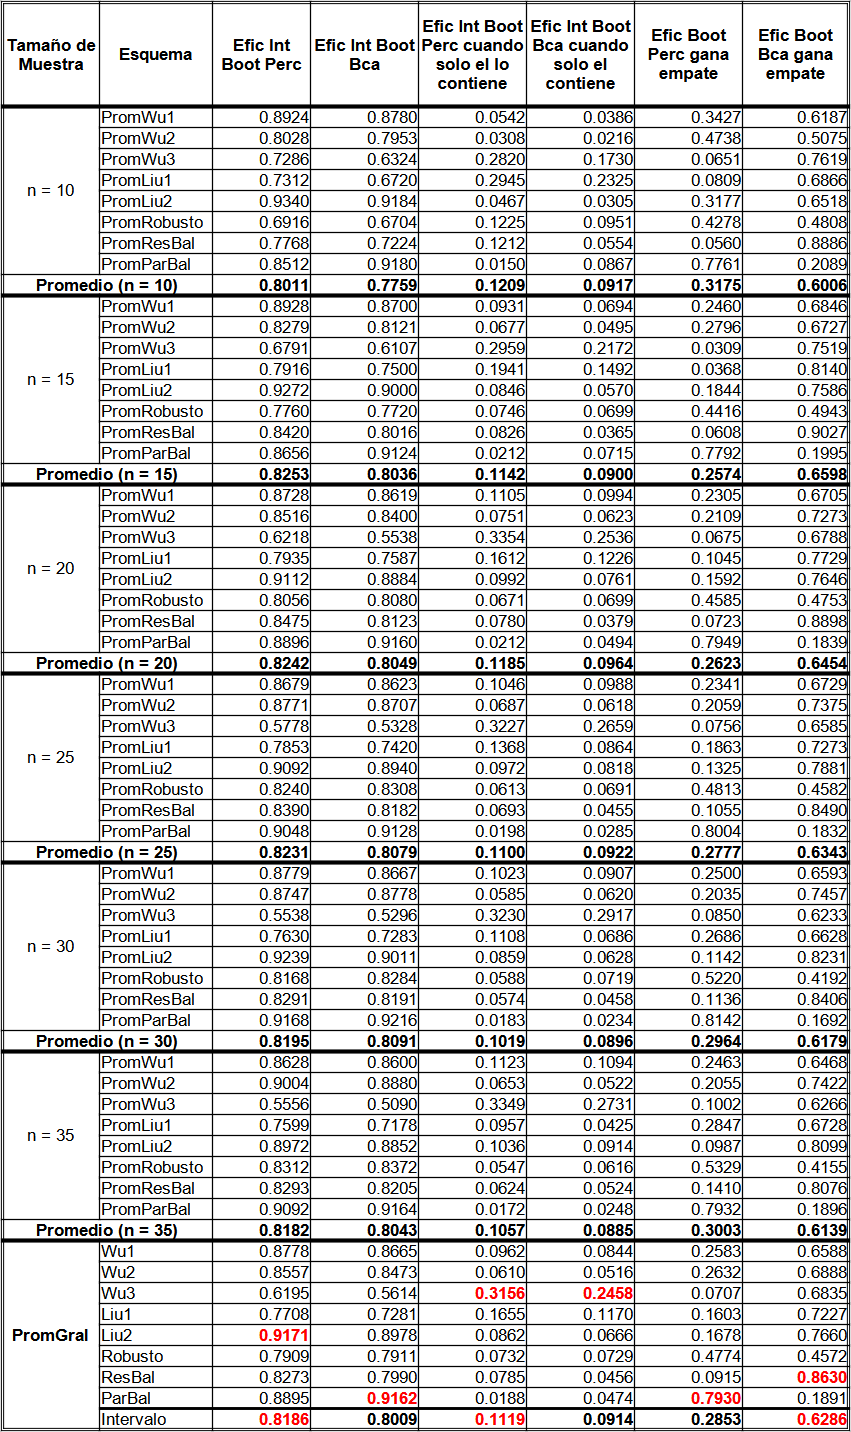
\includegraphics[width=0.55\linewidth]{img/EP_NNVD_Efic_Boots.png} 
	\caption{Eficiencia promedio de los intervalos Bootstrap por tamaño de muestra y esquema de remuestreo para el caso EP-NNVD.} 
	\label{fig:EficPromIntBootsTamMuestEsqRemuEP-NNVD}
\end{figure}
\FloatBarrier

\subsubsection{Eficiencia de los esquemas para el caso EP-NNVD}
Con base en al menos 95\% de eficiencia promedio y sin importar el ICB  (Figura \ref{fig:EficPromEsqTamMuesEsqRemuEP-NNVD}): sólo con el $n=30$ se cumple la condición bajo el esquema Pareado Balanceado (ParBal) con 0.9. Ahora sin considerar el criterio anterior, el mejor esquema para: n=10 es Liu2 (0.8904) y Wu1(0.8440), n=15 es Liu2 (0.8488) y ParBal (0.8472), n=20 es ParBal (0.8708) y Liu2 (0.8207), n=25 es ParBal (0.8868) y Liu2 (0.8207), n=30 es ParBal (0.9) y Liu2 (0.8447) y en n=35 es ParBal (0.8936) y Wu2 (0.8415). \\


Sin considerar el tamaño de la muestra, para el caso EP-NNVD los mejores promedios generales (Figura \ref{fig:EficPromEsqTamMuesEsqRemuEP-NNVD}) en eficiencia de esquema son ParBal (0.8728) y Liu2 (0.8383).


\begin{figure}[ht] 
	\centering 
	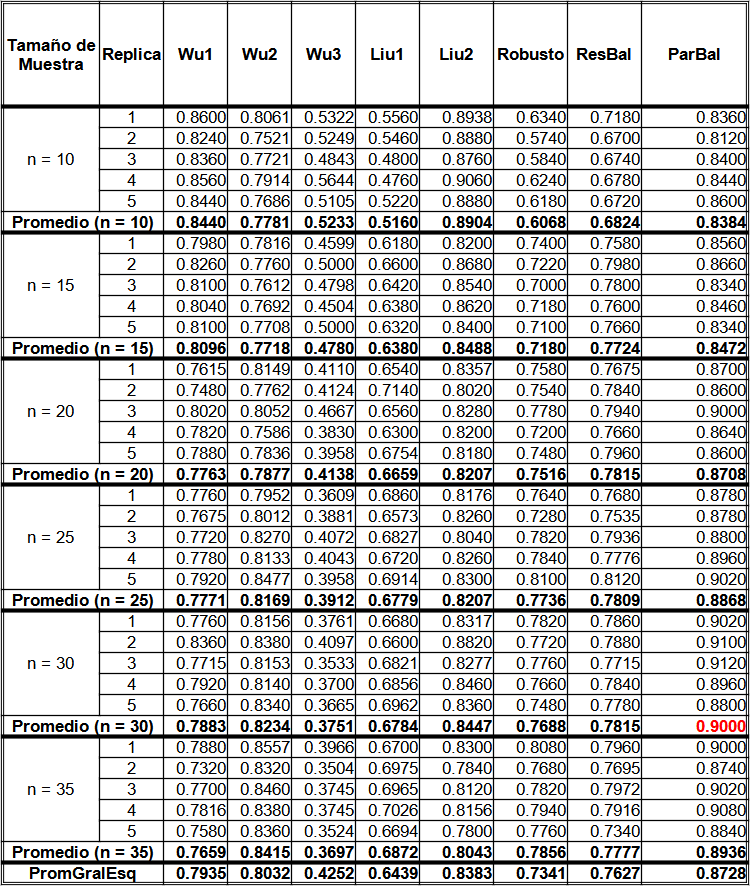
\includegraphics[width=0.70\linewidth]{img/EP_NNVD_Efic_Esq.png} 
	\caption{Eficiencia promedio de los esquemas por tamaño de muestra para el caso EP-NNVD.} 
	\label{fig:EficPromEsqTamMuesEsqRemuEP-NNVD}
\end{figure}
\FloatBarrier

%%Tipo de intervalo y esquema para evaluar la precision. 8 recomendaciones

%%%%%%%%%%%%%%%%%%%

\subsection{Eficiencia promedio por supuestos para el caso EP}
Dados los modelos de tipo EP para los casos: NVC, NNVC y NVD, con base en los promedios generales sin importar el tamaño de muestra (Figura \ref{fig:PromSupuUtiliEP}), por encima del 95\% se recomienda el uso del esquema Liu2 con el intervalo Percentil; y por encima del 90\% para NNVD de igual forma el esquema Liu2 o ParBa pero con el intervalo BCa, para la evaluación de la precisión.


\begin{figure}[ht] 
	\centering 
	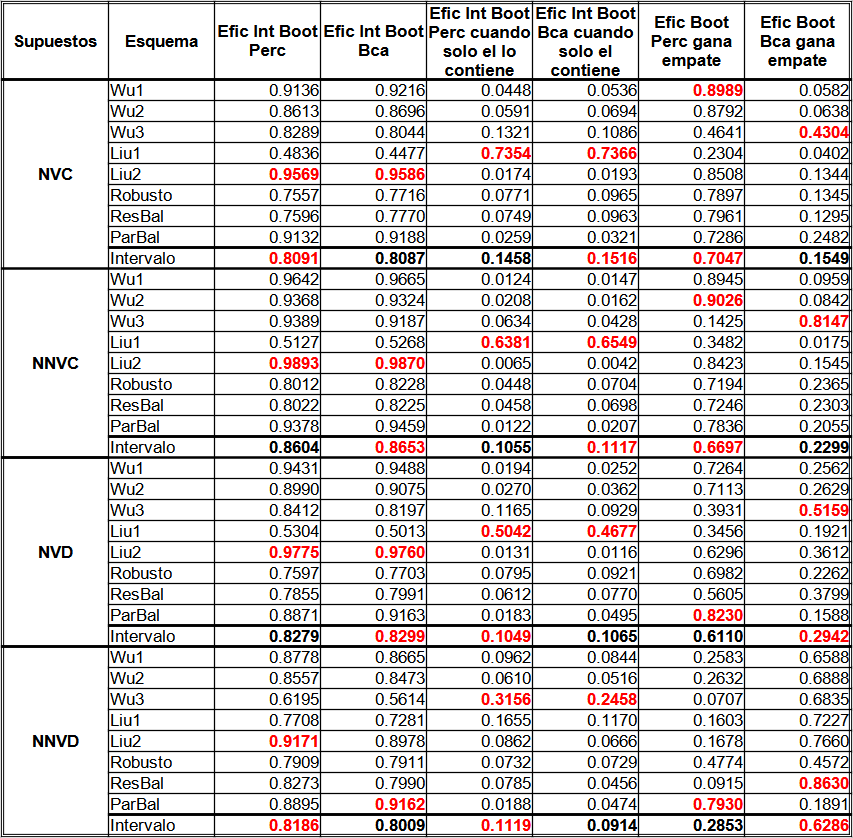
\includegraphics[width=0.80\linewidth]{img/EP_Prom_Supuestos.png} 
	\caption{Eficiencia promedio por supuesto para el caso EP.} 
	\label{fig:PromSupuUtiliEP}
\end{figure}
\FloatBarrier



%%%%%%%%%%%%%%%%%%%%%%%%%%%%%%%%%%%%%%%%%%%%%%%%%%%%%%%%%%%%%%%%%%%%%%%%%%%%%%%%%%%%%%%%%%%

%%%%%%%%%%%%%%%%%%%%%%%%%%%%%%Empieza EI

Análisis descriptivos similares se realizaron para modelos EI (Anexo A). A continuación, y a modo de resumen se presenta el concentrado de eficiencias promedio por cada supuesto sin importar el tamaño de muestra.\\


\subsection{Eficiencia promedio por supuesto para el caso EI}

Dados los modelos de tipo EI para los casos: NVC, NNVC, NVD y NNVD con base en los promedios generales (Figura \ref{fig:PromSupuUtiliEI}), por encima del 95\% se recomienda el uso del esquema Liu 2 con el intervalo BCa, para la evaluación de la precisión.


\begin{figure}[ht] 
	\centering 
	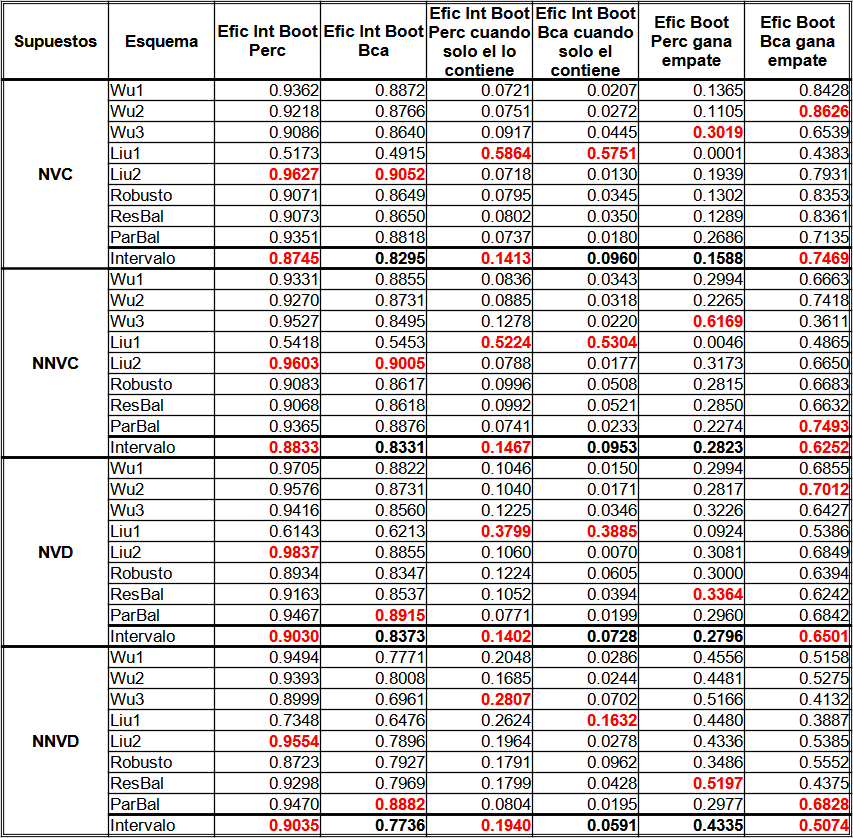
\includegraphics[width=0.80\linewidth]{img/EI_Prom_Supuestos.png} 
	\caption{Eficiencia promedio por supuesto para el caso EI.} 
	\label{fig:PromSupuUtiliEI}
\end{figure}




%%%%%%%%%%%%%%%%%%%%%%%%%%%%%%%%%%%%%%%%%%%%%%%%%%%%%%%%%%%%%%%%%%%%%%%%
%%%%%%%%%%%%%%%%%%%%%Estadistica fuerte

A continuación, los resultados de los análisis estadísticos cuando se tiene cada uno de los casos de supuestos.\\

\subsection{Comparación de la eficiencia del ICB Percentil cuando se tiene NVC (NVC-EficIB1)}

Cuando se tiene NVC y se utilizó el ICB Percentil para evaluar la precisión, se obtuvo interacción triple significativa ($TipoMod \times TM \times Esq: F=11.97, P<0.0001$; Figura \ref{fig:ANOVA_Efic_ICB_Perc_NVC} del Anexo B ). Con base en una eficiencia promedio de al menos 95\%, el mejor esquema resultó Liu2 sin importar el tamaño de muestra y tipo de modelo (Figura \ref{fig:CompEfic_PromICB_Perc_NVC}).\\


\begin{figure}[ht] 
	\centering 
	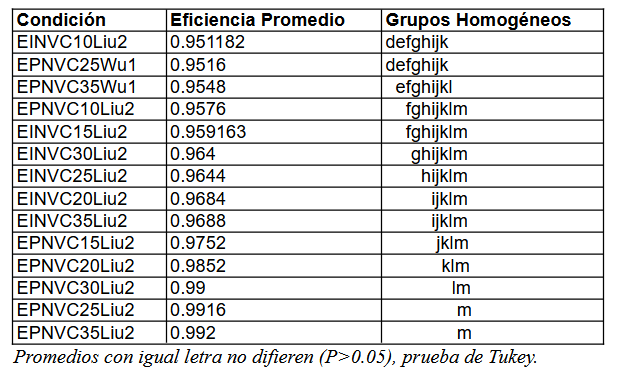
\includegraphics[width=0.76\linewidth]{img/CompEfic_PromICB_Perc_NVC.png} 
	\caption{Comparación de eficiencias promedio del ICB Percentil cuando se tiene NVC.} 
	\label{fig:CompEfic_PromICB_Perc_NVC}
\end{figure}
\FloatBarrier



\subsubsection{Comparación de la eficiencia del ICB BCa cuando se tiene NVC (NVC-EficIB2)}

Cuando se tiene NVC y se utilizó el ICB BCa para evaluar la precisión, se obtuvo interacción triple significativa ($TipoMod \times TM \times Esq: F=3.60, P<0.0001;$ Figura \ref{fig:ANOVA_Efic_ICB_BCa_NVC} del Anexo B). Con base en una eficiencia promedio de al menos 95\%, el mejor esquema resultó Liu2 sin importar el TM, sin embargo, sólo identifica al tipo de modelo EP \textit{a priori} simulado (Figura \ref{fig:CompEfic_PromICB_BCa_NVC}).\\



\begin{figure}[ht] 
	\centering 
	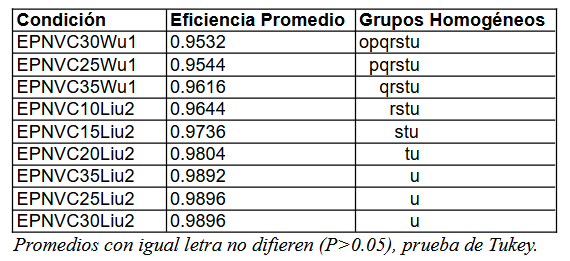
\includegraphics[width=0.76\linewidth]{img/CompEfic_PromICB_BCa_NVC.png} 
	\caption{Comparación de eficiencias promedio del ICB BCa cuando se tiene NVC.} 
	\label{fig:CompEfic_PromICB_BCa_NVC}
\end{figure}
\FloatBarrier



%%%%%%%%%%%%%%%%%%%%%%%%%%%5

\subsection{Comparación de la eficiencia del ICB Percentil cuando se tiene NNVC (NNVC-EficIB1)}

Cuando se tiene NNVC y se utilizó el ICB Percentil para evaluar la precisión, se obtuvo interacción triple significativa ($TipoMod \times TM \times Esq: F=17.86, P<0.0001$; Figura \ref{fig:ANOVA_Efic_ICB_Perc_NNVC} del Anexo B). Con base en una eficiencia promedio de al menos 95\%, el mejor esquema resultó Liu2 sin importar el tamaño de muestra y tipo de modelo; con excepción del caso EINNVC10Liu2, sin embargo, su eficiencia promedio es 94.52\% (Figura \ref{fig:CompEfic_PromICB_Perc_NNVC}).\\

\begin{figure}[ht] 
	\centering 
	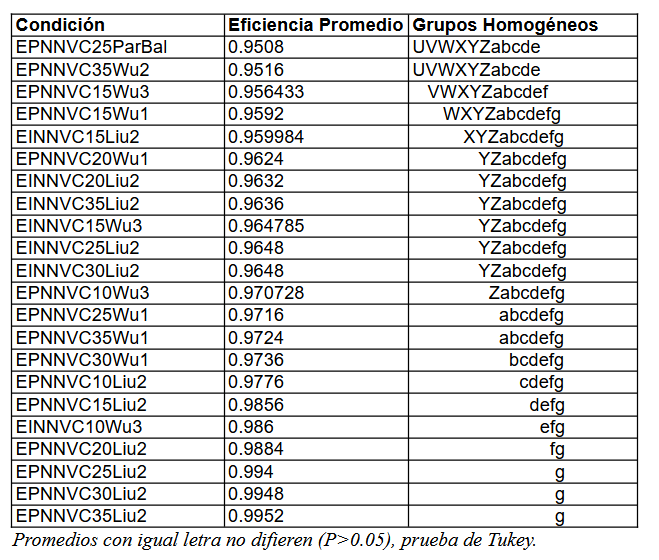
\includegraphics[width=0.76\linewidth]{img/CompEfic_PromICB_Perc_NNVC.png} 
	\caption{Comparación de eficiencias promedio del ICB Percentil cuando se tiene NNVC.} 
	\label{fig:CompEfic_PromICB_Perc_NNVC}
\end{figure}
\FloatBarrier



\subsubsection{Comparación de la eficiencia del ICB BCa cuando se tiene NNVC (NNVC-EficIB2)}

Cuando se tiene NNVC y se utilizó el ICB BCa para evaluar la precisión, se obtuvo interacción triple significativa ($TipoMod \times TM \times Esq: F=5.95, P<0.0001$; Figura \ref{fig:ANOVA_Efic_ICB_BCa_NNVC} del Anexo B). Con base en una eficiencia promedio de al menos 95\%, se obtuvo dos mejores esquemas Liu2 y Wu1 sin importar el TM, sin embargo, ambos sólo identifican al tipo de modelo EP a priori simulado (Figura \ref{fig:CompEfic_PromICB_BCa_NNVC}). \\


\begin{figure}[ht] 
	\centering 
	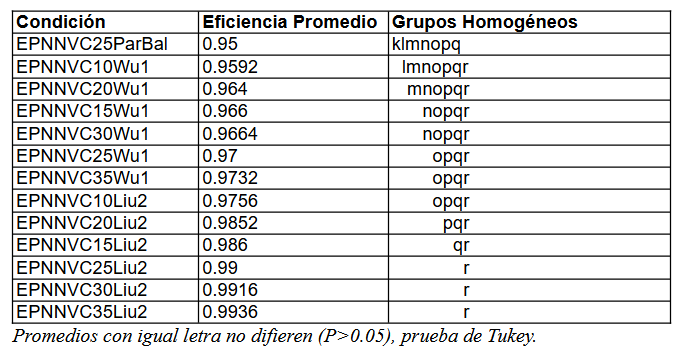
\includegraphics[width=0.76\linewidth]{img/CompEfic_PromICB_BCa_NNVC.png} 
	\caption{Comparación de eficiencias promedio del ICB BCa cuando se tiene NNVC.} 
	\label{fig:CompEfic_PromICB_BCa_NNVC}
\end{figure}
\FloatBarrier




%%%%%%%%%%%%%%%%%%%%%%%%%%%5
\subsection{Comparación de la eficiencia del ICB Percentil cuando se tiene NVD (NVD-EficIB1)}

Cuando se tiene NVD y se utilizó el ICB Percentil para evaluar la precisión, se obtuvo interacción triple significativa ($TipoMod \times TM \times Esq: F=7.89, P<0.0001;$ Figura \ref{fig:ANOVA_Efic_ICB_Perc_NVD} del Anexo B). Con base en una eficiencia promedio de al menos 95\%, el mejor esquema resultó Liu2 sin importar el tamaño de muestra y tipo de modelo (Figura \ref{fig:CompEfic_PromICB_Perc_NVD}).\\


\begin{figure}[ht] 
	\centering 
	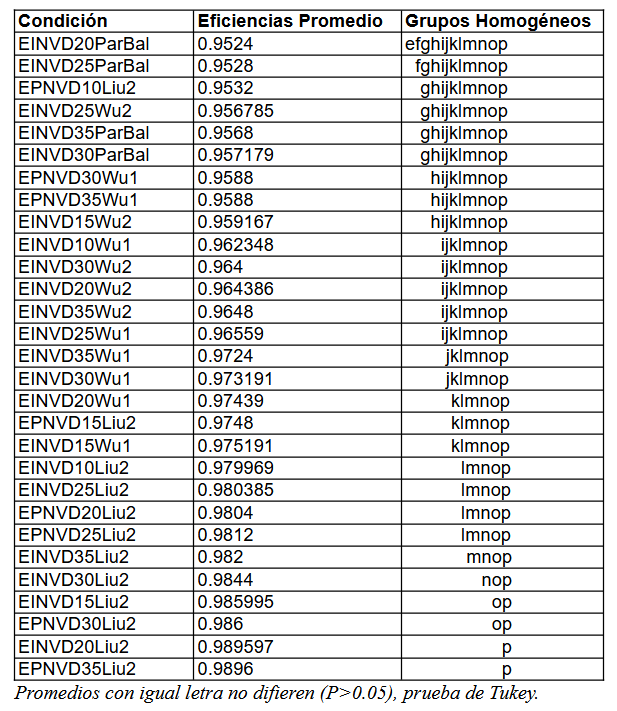
\includegraphics[width=0.76\linewidth]{img/CompEfic_PromICB_Perc_NVD.png} 
	\caption{Comparación de eficiencias promedio del ICB Percentil cuando se tiene NVD.} 
	\label{fig:CompEfic_PromICB_Perc_NVD}
\end{figure}
\FloatBarrier


\subsubsection{Comparación de la eficiencia del ICB BCa cuando se tiene NVD (NVD-EficIB2)}

Cuando se tiene NVD y se utilizó el ICB BCa para evaluar la precisión, se obtuvo interacción triple significativa ($TipoMod \times TM \times Esq: F=3.91, P<0.0001;$ Figura \ref{fig:ANOVA_Efic_ICB_BCa_NVD} del Anexo B). Con base en una eficiencia promedio de al menos 95\%, el mejor esquema resultó Liu2 sin importar el TM, sin embargo, sólo identifica al tipo de modelo EP \textit{a priori} simulado (Figura \ref{fig:CompEfic_PromICB_BCa_NVD})).\\

\begin{figure}[ht] 
	\centering 
	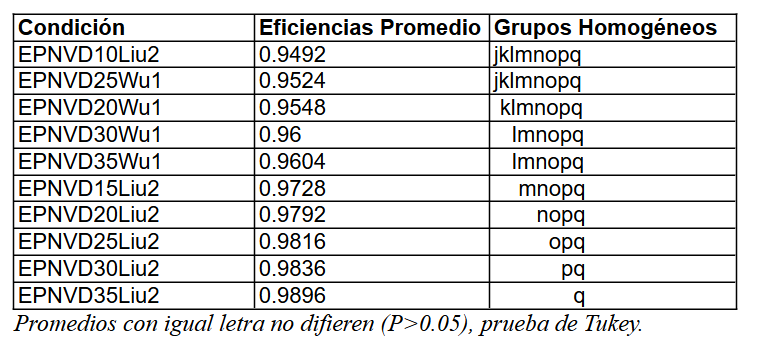
\includegraphics[width=0.76\linewidth]{img/CompEfic_PromICB_BCa_NVD.png} 
	\caption{Comparación de eficiencias promedio del ICB BCa cuando se tiene NVD.} 
	\label{fig:CompEfic_PromICB_BCa_NVD}
\end{figure}
\FloatBarrier



%%%%%%%%%%%%%%%%%%%%%%%%%%%5
\subsection{Comparación de la eficiencia del ICB Percentil cuando se tiene NNVD (NNVD-EficIB1)}

Cuando se tiene NNVD y se utilizó el ICB Percentil para evaluar la precisión, se obtuvo interacción triple significativa ($TipoMod \times TM \times Esq: F=10.71, P<0.0001;$ Figura \ref{fig:ANOVA_Efic_ICB_Perc_NNVD} del Anexo B). Con base en una eficiencia promedio de al menos 93.96\%, se obtuvo dos mejores esquemas Liu2 y ParBal para todos los tamaños de muestra con excepción de n=35 para Liu2 (92.72\%) y n=10 para ParBal (91.28\%). Sin embargo, ambos esquemas sólo identifican al tipo de modelo EI \textit{a priori} simulado (Figura \ref{fig:CompEfic_PromICB_Perc_NNVD}).

\begin{figure}[ht] 
	\centering 
	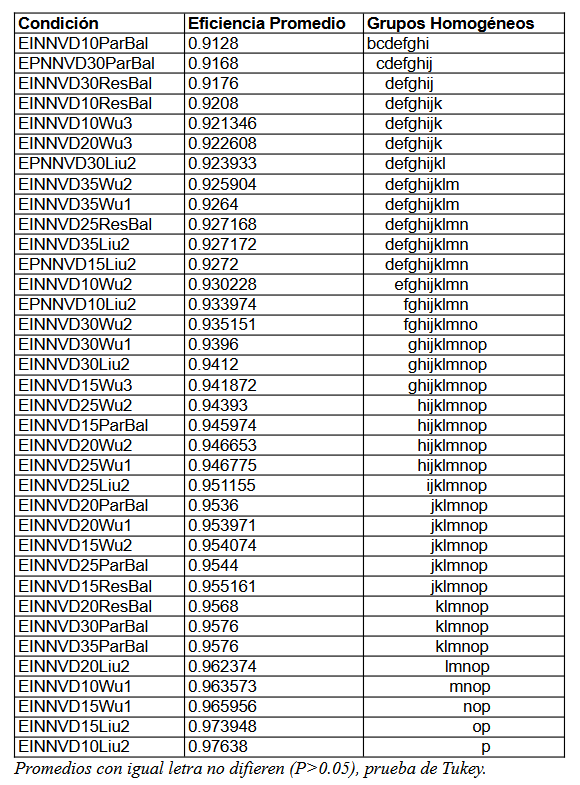
\includegraphics[width=0.76\linewidth]{img/CompEfic_PromICB_Perc_NNVD.png} 
	\caption{Comparación de eficiencias promedio del ICB Percentil cuando se tiene NNVD.} 
	\label{fig:CompEfic_PromICB_Perc_NNVD}
\end{figure}
\FloatBarrier




\subsubsection{Comparación de la eficiencia del ICB BCa cuando se tiene NNVD (NNVD-EficIB2)}

Cuando se tiene NNVD y se utilizó el ICB BCa para evaluar la precisión, se obtuvo interacción triple significativa ($TipoMod \times TM \times Esq: F=11.76, P<0.0001;$ Figura \ref{fig:ANOVA_Efic_ICB_BCa_NNVD} del Anexo B). Con base en una eficiencia promedio de al menos 88.80\%, con el esquema ParBal se obtuvo la mayor eficiencia promedio en todos los tamaños de muestra, también bajo el esquema Liu2 con excepción de $n=35$ (88.52\%) cuando el tipo de modelo a priori simulado es EP. Cabe señalar que el esquema ParBal identifica el tipo de modelo EI para n=25, 30, 35 y las eficiencias no difieren estadísticamente con al menos 90.4\% (Figura \ref{fig:CompEfic_PromICB_BCa_NNVD}).\\


\begin{figure}[ht] 
	\centering 
	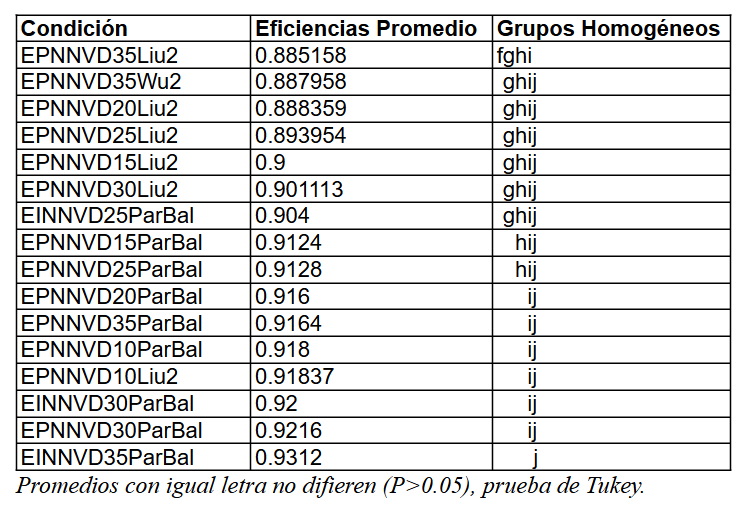
\includegraphics[width=0.76\linewidth]{img/CompEfic_PromICB_BCa_NNVD.png} 
	\caption{Comparación de eficiencias promedio del ICB BCa cuando se tiene NNVD.} 
	\label{fig:CompEfic_PromICB_BCa_NNVD}
\end{figure}
\FloatBarrier



\newpage

\subsection{Propuesta Final}

Con base en los resultados de los análisis estadísticos, cuando se tenga NVC, NNVC o NVD y se evalué la precisión el ICB a utilizar sería Percentil con esquema de remuestreo Liu2. Y cuando se tenga NNVD y se evalué la precisión, el ICB a utilizar sería BCa con esquema de remuestreo Pareado Balanceado.


\subsubsection{Implementación}


Para la propuesta final de este trabajo, dado los resultado estadísticos, para los diferentes casos NVC, NNVC y NVD, se calcula el ICB Percentil para evaluar la precisión con el esquema de Liu2, ya que este obtuvo en el estudio de simulación una eficiencia al menos del 95\%; con las diferencias en la implementación de los residuales: para el caso 1 (NVC) se utilizó los residuales al correr una regresión lineal simple, para el caso 2 (NVD) se utilizó los residuales robustos ponderados y en el caso 3 (NNVC) los residuales robustos sin ponderar. Ademas, cuando se tenga el caso 4 (NNVD) se evalúa la precisión con el ICB BCa con el esquema de remuestreo Pareado Balanceado que obtuvo una eficiencia al menos del 88.8\%.\\

La propuesta final se implementó con el lenguaje R, de tal forma que la evaluación de la precisión se realiza de manera automática dependiendo del cumplimiento de los supuestos. En las salidas, se presentan los resultados de las pruebas estadísticas junto con su conclusión respectiva y en el ICB para $R^2$ se presentan los límites inferior (LI) y superior (LS) estimados junto con la conclusión de si el modelo evaluado es preciso o impreciso bajo el criterio: $LI \leq  70  \leq LS \; o \; LI \geq 70\%$.\\



Los argumentos necesarios en la función de la propuesta final, son: la muestra bivariada $(z_1, y_1), (z_2, y_2), \dots, (z_n, y_n)$ formada por los predichos $z_i$ y por los observados $y_i$ del modelo a evaluar y un nivel del confianza $1-\alpha$ para el ICB, de modo que nivel de significancia $\alpha$ para las pruebas estadísticas se determina a partir del coeficiente de confianza. La figura \ref{fig:propuestaFinal}  muestra el diagrama de flujo de la propuesta final y en el Anexo C7 se encuentra el script de R correspondiente a la función \textit{EvaluaPrecICB()}.

\begin{figure}[ht!]
	\centering 
	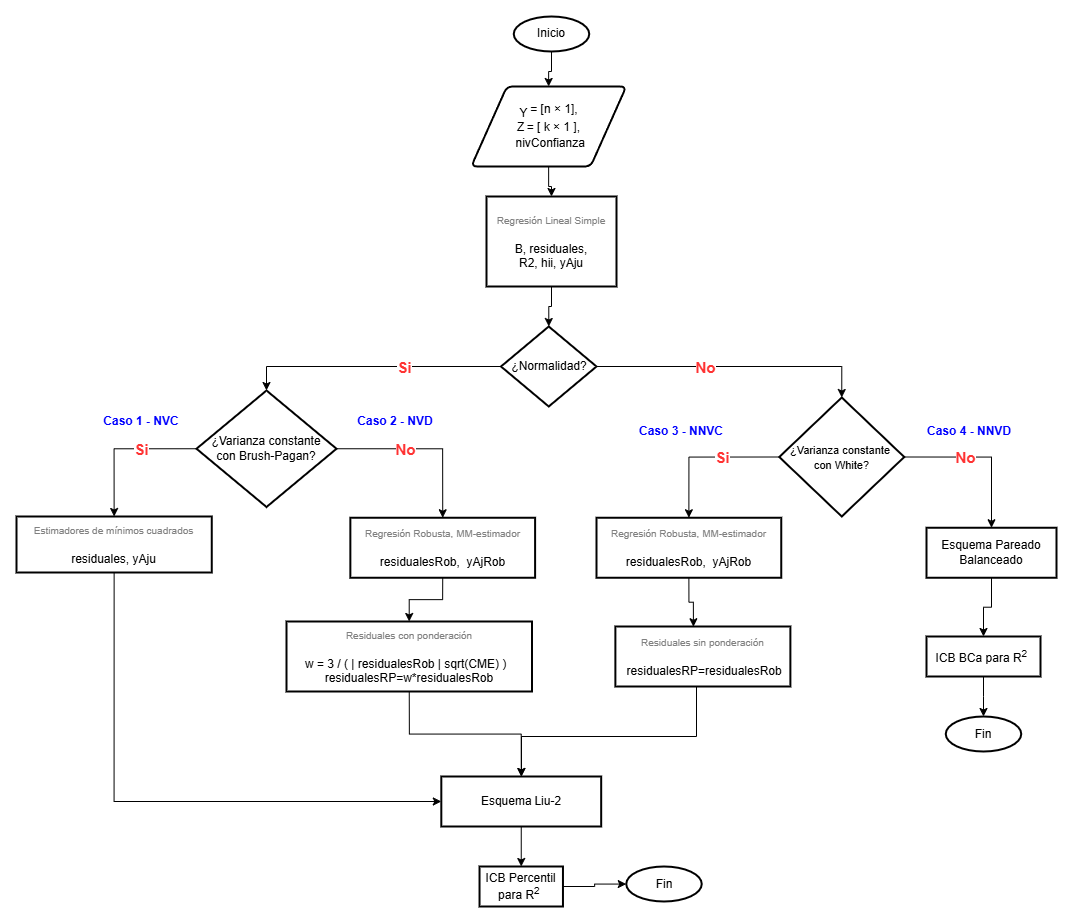
\includegraphics[width=0.94\linewidth]{img/propuestaFinalv7.png} 
	\caption{Diagrama de flujo de la propuesta final para evaluar la precisión de un modelo.}
	\label{fig:propuestaFinal}
\end{figure}
\FloatBarrier

\clearpage

\newpage

\subsubsection{Aplicación}

\textbf{Caso 1 - NVC}

Para este caso se consideraron los datos experimentales de la ganancia diaria de peso (GDP) en ovinos; datos experimentales vs. modelo de simulación para estimar la ganancia diaria de peso (GDP) \parencite{osorio-2011}. Estos datos se encuentran en el apéndice B de \textcite{balam-2012}.\\


Utilizando 95\% de coeficiente de confianza y con base en los resultados al verificar los supuestos (Figura \ref{fig:final_NVC_resultados}) se obtuvo que corresponde al caso NVC. Por lo tanto, en la evaluación de la precisión se aplicó el ICB Percentil con el esquema de remuestreo Liu2, dando como resultado que el modelo evaluado es preciso considerando un $R^2 \geq 70\%$.Es decir, se cumplió que el ICB estimado para $R^2$ contiene el valor 70\%.


\begin{figure}[ht!]
	\centering 
	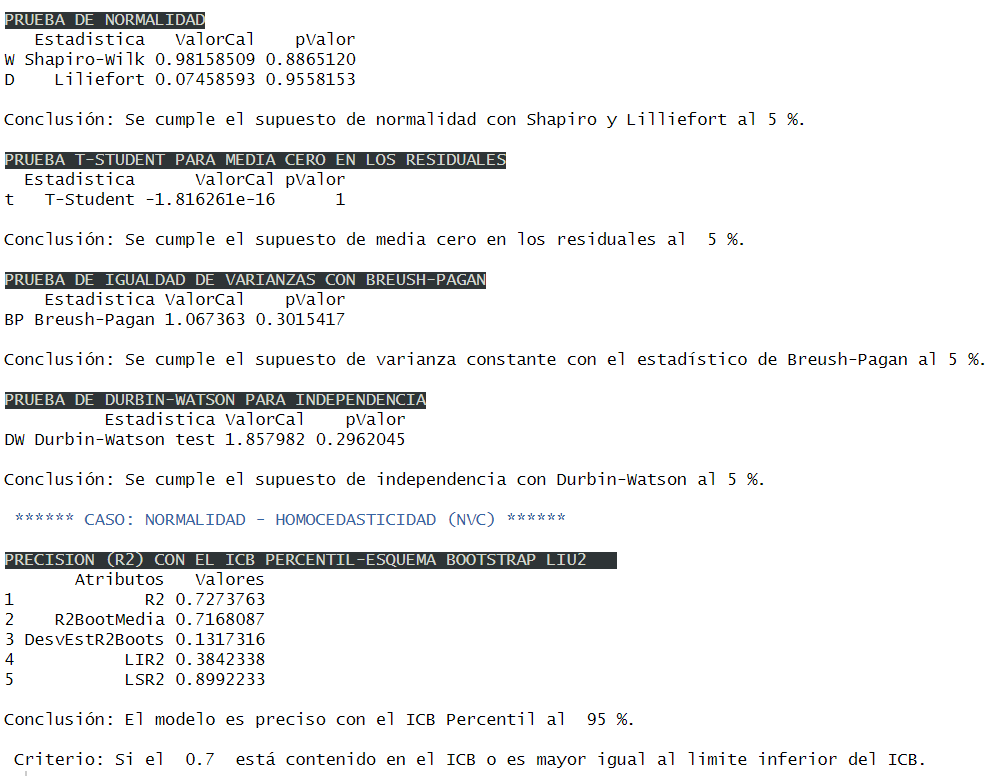
\includegraphics[width=0.9\linewidth]{img/Uso_NVC_PropuestaFinal.png} 
	\caption{Resultados del caso NVC.}
	\label{fig:final_NVC_resultados}
\end{figure}
\FloatBarrier
\clearpage

\newpage

\textbf{Caso 2 - NNVD}\\
Se aplicó a los datos experimentales del volumen de una parcela en metros cúbicos a un diámetro superior $(n = 63)$ de 10cm y los simulados con el modelo PTAEDA \parencite{chung-1987}, el cual es un modelo estocástico. Cada simulación con el modelo PTAEDA corresponde a la media de 10 corridas del modelo para cada parcela. En cada parcela se mide la edad, el indice de sitio y el número de arboles por hectárea. Estos datos se encuentran en el apéndice B de \textcite{balam-2012}.\\


Utilizando 95\% de coeficiente de confianza y con base en los resultados al verificar los supuestos (Figura \ref{fig:final_NNVD_resultados}) se obtuvo que corresponde al caso NNVD. Por lo tanto, en la evaluación de la precisión se aplicó el ICB BCa con el esquema de remuestreo Pareado Balanceado, dando como resultado que el modelo evaluado es preciso considerando un $R^2 \geq 70\%$. Es decir, se cumplió que el $LI$ estimado
para $R^2$ es mayor que 70\%.

\begin{figure}[ht!]
	\centering 
	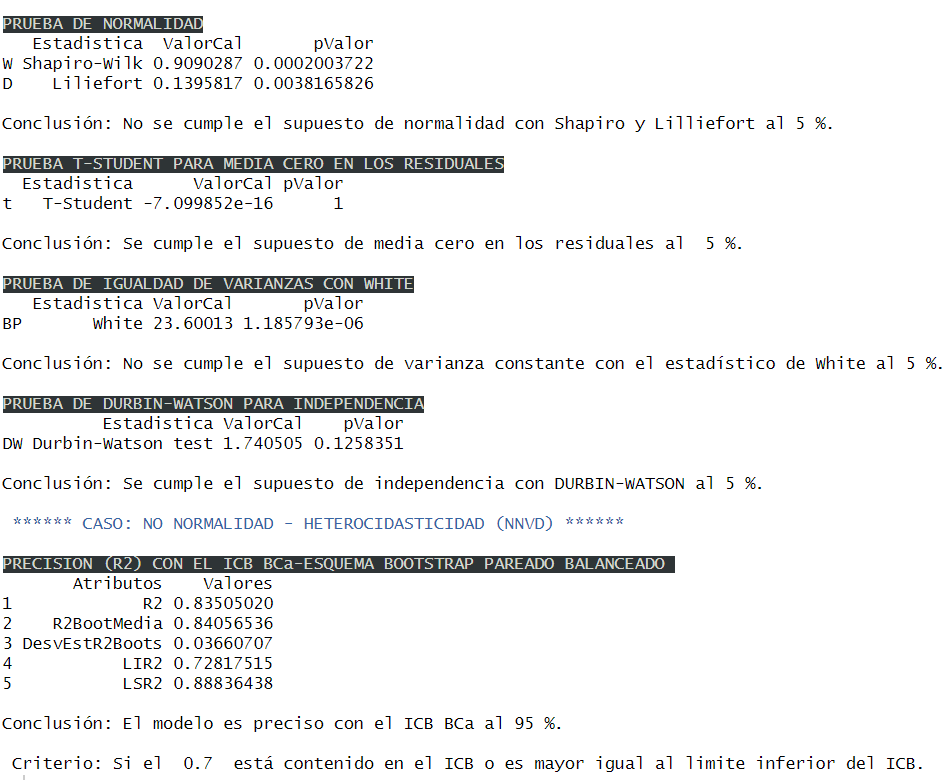
\includegraphics[width=0.9\linewidth]{img/Uso_NNVD_PropuestaFinal.png} 
	\caption{Resultados del caso NNVD.}
	\label{fig:final_NNVD_resultados}
\end{figure}

\FloatBarrier % Asegura que los floats no pasen esta línea
\clearpage
